% !TeX program = xelatex
\documentclass[10pt,a4paper]{ctexart} % 设置文章类型，正文字号与纸张大小

% 页面与正文常用宏包
\usepackage[margin=2cm]{geometry} % 设置页面四周页边距
\usepackage{graphicx}             % 插入图片
\usepackage{amsmath}              % 提供cases、aligned等数学公式环境
\usepackage{amssymb}              % 提供\therefore等扩展数学符号
\usepackage{booktabs}             % 提供\toprule、\midrule、\bottomrule三线表命令
\usepackage{float}                % 提供[H]固定图片、表格位置
\usepackage{subcaption}           % 提供subfigure子图环境及子图标题
\usepackage{wrapfig}              % 提供wrapfigure图文环绕环境
\usepackage{fancyhdr}             % 自定义页眉和页脚
\usepackage{hyperref}             % 生成超链接

% 页眉页脚
\pagestyle{fancy}                  % 启用fancyhdr定义的页面样式
\fancyhf{}                         % 清空默认页眉和页脚
\fancyfoot[C]{\thepage}            % 在页脚中央显示页码
\renewcommand{\headrulewidth}{0pt} % 隐藏页眉横线
\renewcommand{\footrulewidth}{0pt} % 隐藏页脚横线

% 超链接
\hypersetup{
  colorlinks=true,                % 使用彩色文字链接，而非带边框的链接
  linkcolor=red,                 % 目录、公式及图表交叉引用的颜色
  filecolor=cyan,                 % 本地文件链接的颜色
  urlcolor=blue,                  % 网址链接的颜色
  pdftitle={分光计的调整和使用+棱镜偏向角特性报告},     % 写入PDF文档属性的标题
  bookmarksnumbered=true          % PDF书签显示章节编号
}

% 定义字号命令
\newcommand{\chuhao}{\fontsize{42pt}{63pt}\selectfont}
\newcommand{\xiaochu}{\fontsize{36pt}{54pt}\selectfont}
\newcommand{\yihao}{\fontsize{26pt}{39pt}\selectfont}
\newcommand{\xiaoyi}{\fontsize{24pt}{36pt}\selectfont}
\newcommand{\erhao}{\fontsize{22pt}{33pt}\selectfont}
\newcommand{\xiaoer}{\fontsize{18pt}{27pt}\selectfont}
\newcommand{\sanhao}{\fontsize{16pt}{24pt}\selectfont}
\newcommand{\xiaosan}{\fontsize{15pt}{22.5pt}\selectfont}
\newcommand{\sihao}{\fontsize{14pt}{21pt}\selectfont}
\newcommand{\xiaosi}{\fontsize{12pt}{18pt}\selectfont}
\newcommand{\wuhao}{\fontsize{10.5pt}{15.75pt}\selectfont}
\newcommand{\xiaowu}{\fontsize{9pt}{13.5pt}\selectfont}

% 章节格式
\ctexset{
  section={
    format={\CJKfontspec[AutoFakeBold=2.5]{KaiTi}\sanhao\bfseries}, % 一级标题使用三号加粗楷体
    name={,、},                                                    % 在中文章节序号后添加顿号
    number=\chinese{section},                                      % 一级标题编号使用“一、二、三”形式
    aftername={}                                                   % 取消编号与标题文字之间的空格
  },
  subsection={
    format={\CJKfontspec[AutoFakeBold=2.5]{KaiTi}\sihao\bfseries}, % 二级标题使用四号加粗楷体                                               
  },
  subsubsection={
    format={\CJKfontspec[AutoFakeBold=2.5]{KaiTi}\xiaosi\bfseries}, % 三级标题使用小四加粗楷体
  }
}

\begin{document}

% 封面
\thispagestyle{fancy} % 封面保留底部居中的页码
\fancyfoot[C]{\thepage}
\begin{center}
  \CJKfontspec[AutoFakeBold=2.5]{KaiTi}\bfseries % 封面中文使用楷体并人工加粗，西文同时加粗
  \vspace{0.8cm}
  
\includegraphics[width=8.2cm]{figures/head.png}

  \vspace{0.2cm}
  \xiaochu 
    物理实验报告

  \vspace{3.5cm}
  \begin{minipage}{14.0cm}
    \sanhao
    \makebox[2.6cm][l]{实验名称：}
    \underline{\makebox[11.0cm][c]{分光计的调整和使用+棱镜偏向角特性}}\par\vspace{12pt}

    \makebox[2.6cm][l]{实验桌号：}
    \underline{\makebox[11.0cm][c]{19}}\par\vspace{12pt}

    \makebox[2.6cm][l]{指导教师：}
    \underline{\makebox[11.0cm][c]{王兆英}}
  \end{minipage}

  \vspace{3.5cm}
  \begin{minipage}{10.0cm}
    \sihao
    \makebox[1.4cm][l]{班级：}
    \underline{\makebox[8.0cm][c]{}}\par\vspace{10pt}

    \makebox[1.4cm][l]{姓名：}
    \underline{\makebox[8.0cm][c]{IllusoryRain}}\par\vspace{10pt}

    \makebox[1.4cm][l]{学号：}
    \underline{\makebox[8.0cm][c]{}}
  \end{minipage}

  \vspace{2.0cm}
  \sihao
    实验日期：
    \underline{\makebox[0.7cm][c]{2026}}年
    \underline{\makebox[0.7cm][c]{10}}月
    \underline{\makebox[1.4cm][c]{21/28}}日
    星期\underline{\makebox[1.4cm][c]{三/三}}上午

  \vspace{0.7cm}
  \sihao 
    浙江大学物理实验教学中心
\end{center}

\newpage
\xiaosi\songti\mdseries % 后续正文统一使用小四不加粗的宋体

\section{预习报告（10分）}

  \subsection{实验综述（5分）}

    \subsubsection{分光计的调整和使用}
    分光计主要由平行光管、望远镜、载物台和读数装置组成。先目测预调，使望远镜、平行光管及载物台大致水平，再进行以下调整：
    \begin{enumerate}
      \item 调节目镜使叉丝清晰，利用双面平面镜进行自准直调节，使反射“十”字像清晰且与叉丝无视差。（可选）
      \item 调整叉丝方向，用“各半调节法”调节望远镜倾斜螺钉和载物台调平螺钉，使平面镜两面的反射像均与上方叉丝重合。
      \item 用望远镜观察平行光管狭缝，调节狭缝位置使像清晰且无视差，再调节光管倾斜及狭缝方向，使狭缝像竖直、居中且宽度适当。
    \end{enumerate}
    
    调整后，平行光管发出平行光，望远镜光轴、平行光管光轴及载物台平面均垂直于仪器主轴。

    本实验采用棱脊分束法测量三棱镜顶角。将待测顶角的棱脊朝向平行光管，
    平行光经构成顶角的两个光学面反射，形成夹角为顶角两倍的左、右两束反射光。
    保持载物台不动，用望远镜分别瞄准两侧反射狭缝像，记录两个位置的双游标读数，顶角为
    \[
    A=\frac{\left|\theta_{\text{右I}}-\theta_{\text{左I}}\right|
           +\left|\theta_{\text{右II}}-\theta_{\text{左II}}\right|}{4}
    \]
    
    其中，“左”“右”表示两侧反射像的位置，I、II表示两个游标。
    读数跨越零刻度时，应先作跨零处理；双游标读数取平均可减小刻度盘偏心引起的误差。

    这样操作是为了消除偏心差，此外读数也有一定要求，具体如下图：
    \begin{figure}[H]
      \centering
      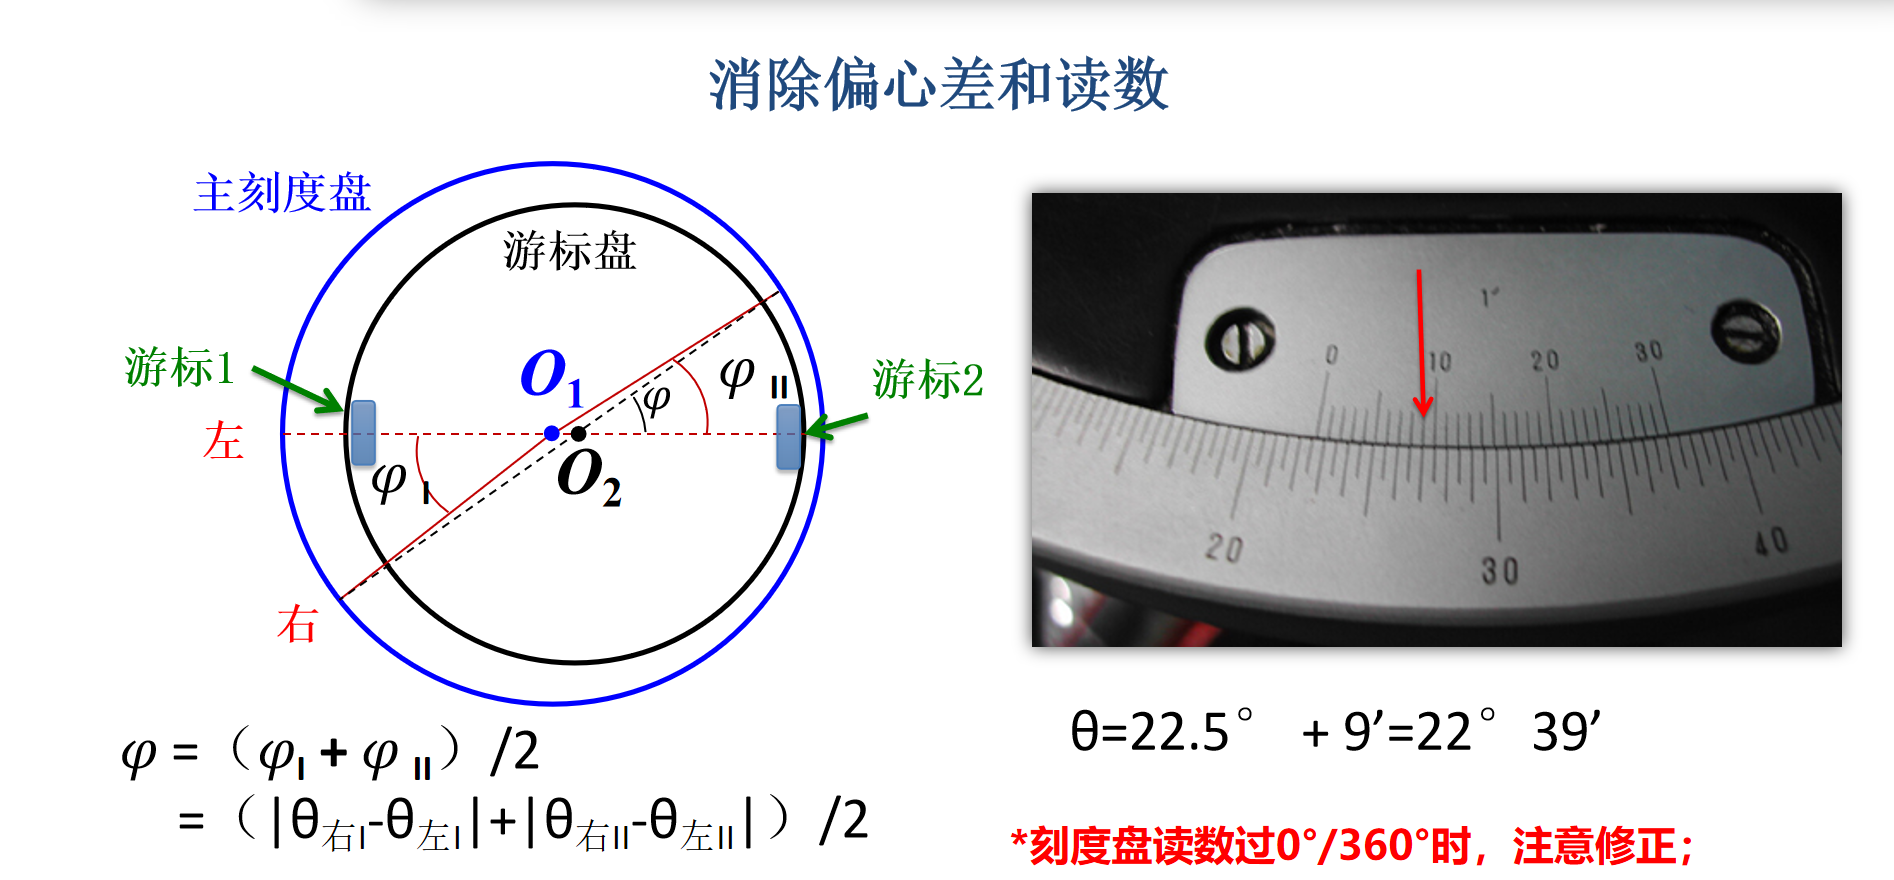
\includegraphics[width=0.65\textwidth]{figures/图1.png}
      \caption{消除偏心差和读数}
    \end{figure}

    综上本实验包括以下内容：
    \begin{enumerate}
      \item 了解分光计的结构。
      \item 用双面平面镜调整分光计。
      \item 用棱脊分束法测量三棱镜顶角。
    \end{enumerate}

    \subsubsection{棱镜偏向角特性}
    光线通过顶角为$A$、折射率为$n$的三棱镜时，由折射定律和几何关系可得
    \[
    \sin i_1=n\sin i_2 \qquad
    \sin i_4=n\sin i_3 \qquad
    i_2+i_3=A
    \]
    \[
    \delta=(i_1-i_2)+(i_4-i_3)=i_1+i_4-A
    \]
    
    其中，$i_1$、$i_4$分别为入射角和出射角，$i_2$、$i_3$为棱镜内的折射角和入射角。

    偏向角$\delta$随入射角增大先减小后增大。令$\dfrac{d\delta}{di_1}=0$，得
    $\dfrac{di_4}{di_1}=-1$；结合折射定律的微分关系及$di_2=-di_3$，可得
    \[
    \frac{\cos i_2}{\cos i_1}=\frac{\cos i_3}{\cos i_4}
    \]
    
    代入折射定律并化简，得$i_2=i_3$，从而$i_1=i_4$。
    此时光路对称，偏向角达到最小值，且
    \[
    i_2=i_3=\frac{A}{2} \qquad
    i_1=i_4=\frac{A+\delta_{\min}}{2}
    \]
    
    因此，测得顶角$A$和最小偏向角$\delta_{\min}$后，即可计算折射率：
    \[
    n=\frac{\sin\left(\dfrac{A+\delta_{\min}}{2}\right)}
           {\sin\left(\dfrac{A}{2}\right)}
    \]

    出射面$AC$的全反射临界角为$C=\arcsin(1/n)$。
    当$A=60^\circ$、$n\approx1.66$时，$C\approx37^\circ$，
    对应$i_2=A-C\approx23^\circ$、$i_1\approx40^\circ$；
    入射角低于该临界值时，光线在$AC$面发生全反射。

    \begin{figure}[H]
      \centering
      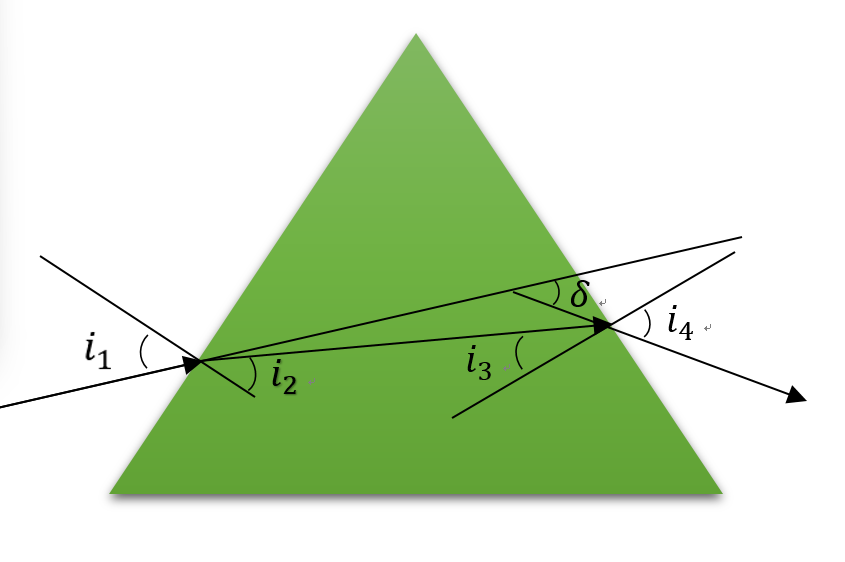
\includegraphics[width=0.4\textwidth]{figures/图2.png}
      \caption{最小偏向角测量原理图}
    \end{figure}

    实验包括以下内容：
    \begin{enumerate}
      \item 调整分光计
      \item 测量三棱镜顶角$A$
      \item 测量最小偏向角$\delta_{\min}$
      \item 计算三棱镜单色光折射率
      \item 绘制色散曲线并思考
    \end{enumerate}

  \subsection{实验重点（3分）}
  
    \subsubsection{分光计的调整和使用}
    \begin{enumerate}
      \item 了解分光计结构、光路和各部分作用
      \item 熟悉示波器面板旋钮的功能，掌握示波器的调节和使用方法。掌握分光计调整和使用
      \item 利用棱脊分束法测量三棱镜顶角
    \end{enumerate}

    \subsubsection{棱镜偏向角特性}
    \begin{enumerate}
      \item 分光计调整和使用
      \item 三棱镜顶角的测量
      \item 测量棱镜的折射率并研究其色散规律
    \end{enumerate}

  \subsection{实验难点（2分）}

    \subsubsection{分光计的调整和使用}
    \begin{enumerate}
      \item 利用双面平面镜调整望远镜与载物台，并调节平行光管，使其出射平行光。
      \item 准确辨认反射像和掠入射位置，正确读取双游标示数并计算角度。
      \item 正确辨认汞灯谱线及衍射级次，准确测量衍射角并计算波长。
    \end{enumerate}

    \subsubsection{棱镜偏向角特性}
    \begin{enumerate}
      \item 合理放置三棱镜，准确瞄准两面的反射像并测量顶角。
      \item 跟踪折射谱线，准确判断其转向位置并测量最小偏向角。
      \item 将各谱线波长与测量数据对应，计算折射率并分析色散曲线。
    \end{enumerate}

\section{实验操作与原始数据（50分）}
% 填写自己的实验数据图

\section{结果与分析（30分）}

  \subsection{数据处理与结果（20分）}  
  
    \subsubsection{分光计的调整和使用}
    实验测得以下数据，并根据公式$
    \angle A =
    \frac{
      |\theta_{\mbox{右}\mathrm{I}}-\theta_{\mbox{左}\mathrm{I}}|
      +
      |\theta_{\mbox{右}\mathrm{II}}-\theta_{\mbox{左}\mathrm{II}}|
    }{4}
    $计算得到以下表格。
    
    注意计算角$A$时：
    分光计刻度盘读数为$0^\circ 0' \sim 359^\circ 59'$，
    当$|\theta_{\mbox{右}\mathrm{I}}-\theta_{\mbox{左}\mathrm{I}}|$
    （或$|\theta_{\mbox{右}\mathrm{II}}-\theta_{\mbox{左}\mathrm{II}}|$）
    大于$180^\circ$时，对较小的读数先加上$360^\circ 0'$，再按公式处理。

    \begin{table}[H]
      \centering
      \caption{三棱镜顶角的测量}
      \begin{tabular}{cccccccc}
        \toprule
          & \multicolumn{2}{c}{方位左} & \multicolumn{2}{c}{方位右} & & & \\
        次数 & 游标I窗 & 游标II窗 & 游标I窗 & 游标II窗 
          & $|\theta_{\mbox{右}\mathrm{I}}-\theta_{\mbox{左}\mathrm{I}}|$ 
          & $|\theta_{\mbox{右}\mathrm{II}}-\theta_{\mbox{左}\mathrm{II}}|$ & $\angle A$ \\
        \midrule
        1 & $45^\circ52'$  & $225^\circ50'$ & $285^\circ58'$ & $105^\circ53'$
          & $119^\circ54'$ & $119^\circ57'$ & $59^\circ58'$ \\
        2 & $50^\circ10'$ & $230^\circ08'$ & $290^\circ10'$ & $110^\circ03'$
          & $120^\circ00'$ & $120^\circ05'$ & $60^\circ01'$ \\
        3 & $33^\circ45'$ & $213^\circ41'$ & $273^\circ45'$ & $93^\circ41'$
          & $120^\circ00'$ & $120^\circ00'$ & $60^\circ00'$ \\
        4 & $71^\circ25'$ & $251^\circ23'$ & $311^\circ31'$ & $131^\circ29'$
          & $119^\circ54'$ & $119^\circ54'$ & $59^\circ57'$ \\
        5 & $48^\circ00'$ & $227^\circ54'$ & $288^\circ03'$ & $108^\circ02'$
          & $119^\circ57'$ & $119^\circ52'$ & $59^\circ57'$ \\
        6 & $27^\circ05'$ & $207^\circ01'$ & $267^\circ10'$ & $87^\circ06'$
          & $119^\circ55'$ & $119^\circ55'$ & $59^\circ58'$ \\
        \bottomrule
      \end{tabular}
    \end{table}

    计算平均值及不确定度时，保留各次顶角的中间计算精度，将角度统一用分表示，六次测量结果分别为：
    \[
    \begin{aligned}
      A_1&=3597.75', & A_2&=3601.25', & A_3&=3600.00',\\
      A_4&=3597.00', & A_5&=3597.25', & A_6&=3597.50'
    \end{aligned}
    \]

    三棱镜顶角的平均值为：
    \[
    \overline{A}=\frac{1}{6}\sum_{i=1}^{6}A_i
    =\frac{21590.75'}{6}
    \approx3598.4583'=59^\circ58.4583'
    \]

    将平均值精确到整数分，则$\overline{A}=59^\circ58'$。

    已知参考角度为$A_0=60^\circ$，则绝对误差为：
    \[
    \Delta A=|\overline{A}-A_0|
    =|59^\circ58.4583'-60^\circ|
    =1.5417'\approx0.02569^\circ
    \]

    相对误差为：
    \[
    E=\frac{\Delta A}{A_0}\times100\%
    =\frac{0.02569^\circ}{60^\circ}\times100\%
    \approx0.0428\%
    \]

    A类标准不确定度为：
    \[
    u_a=\sqrt{\frac{1}{n(n-1)}\sum_{i=1}^{n}(A_i-\overline{A})^2},
    \qquad n=6
    \]

    将各次测量结果代入，得到：
    \[
    \sum_{i=1}^{6}(A_i-\overline{A})^2
    \approx15.1771\,(1')^2
    \]
    
    因此：
    \[
    u_a=\sqrt{\frac{15.1771}{6\times5}}\times1'
    \approx0.7113'
    \]

    仪器允差为 $\Delta_{\mbox{仪}}=1'$，按均匀分布计算
    B类标准不确定度：
    \[
    u_b=\frac{\Delta_{\mbox{仪}}}{\sqrt{3}}
    =\frac{1'}{\sqrt{3}}\approx0.5774'
    \]

    合成标准不确定度为：
    \[
    u_c=\sqrt{u_a^2+u_b^2}
    \approx\sqrt{(0.7113')^2+(0.5774')^2}
    \approx0.9161'
    \]

    按课堂要求，将合成不确定度向上进位保留至整数分，得到 $u_c=1'$，
    平均值相应修约至整数分，最终测量结果为：
    \[
    \boxed{\angle A=59^\circ58'\pm1'}
    \]

    \subsubsection{棱镜偏向角特性}
    实验先测量三棱镜对汞灯绿光的最小偏向角。
    
    其中最小偏向角根据公式
    $\delta_{\min} = \frac{1}{2}\left(\left|\varphi_1 - \varphi_{10}\right| + \left|\varphi_2 - \varphi_{20}\right|\right)$
    计算得到，共测六组，得到以下表格：
    \begin{table}[H]
      \centering
      \caption{绿光的最小偏向角}
      \begin{tabular}{cccccc}
        \toprule
          & \multicolumn{2}{c}{折射关系} & \multicolumn{2}{c}{入射光线} & \\
        次数 & 游标I窗 & 游标II窗 & 游标I窗 & 游标II窗 & $\text{最小偏向角}\,\delta_{\min}$ \\
        \midrule
        1 & $321^\circ48'$ & $141^\circ43'$ & $270^\circ21'$ & $90^\circ21'$ & $51^\circ25'$ \\
        2 & $320^\circ10'$ & $140^\circ08'$ & $268^\circ50'$ & $88^\circ50'$ & $51^\circ19'$ \\
        3 & $316^\circ35'$ & $136^\circ32'$ & $265^\circ10'$ & $85^\circ11'$ & $51^\circ23'$ \\
        4 & $314^\circ25'$ & $134^\circ21'$ & $262^\circ55'$ & $82^\circ51'$ & $51^\circ30'$ \\
        5 & $323^\circ51'$ & $143^\circ46'$ & $272^\circ28'$ & $92^\circ29'$ & $51^\circ20'$ \\
        6 & $323^\circ55'$ & $143^\circ49'$ & $272^\circ28'$ & $92^\circ28'$ & $51^\circ24'$ \\
        \bottomrule
      \end{tabular}
    \end{table}

    计算平均值及不确定度时保留中间计算精度。第1次最小偏向角的未修约值为$51^\circ24.5'$，表中已修约至整数分。
    将六次结果统一用分表示，得到：
    \[
    \begin{aligned}
      \delta_1&=3084.5', & \delta_2&=3079.0', & \delta_3&=3083.0',\\
      \delta_4&=3090.0', & \delta_5&=3080.0', & \delta_6&=3084.0'
    \end{aligned}
    \]

    根据公式，绿光最小偏向角的平均值为：
    \[
    \overline{\delta}_{\min}
    =\frac{1}{6}\sum_{i=1}^{6}\delta_i
    =\frac{18500.5'}{6}
    \approx3083.4167'=51^\circ23.4167'
    \]
    
    将平均值精确到整数分，则$\overline{\delta}_{\min}=51^\circ23'$。

    接下来计算最小偏向角的不确定度，根据公式，A类不确定度为：
    \[
    u_a=\sqrt{\frac{\sum_{i=1}^{6}
    (\delta_i-\overline{\delta}_{\min})^2}{6\times5}}
    =\sqrt{\frac{76.2083}{30}}\times1'
    \approx1.5938'
    \]

    沿用三棱镜顶角测量中仪器允差$\Delta_{\mbox{仪}}=1'$，B类不确定度为：
    \[
    u_b=\frac{\Delta_{\mbox{仪}}}{\sqrt{3}}
    =\frac{1'}{\sqrt{3}}\approx0.5774'
    \]

    合成标准不确定度为：
    \[
    u_c=\sqrt{u_a^2+u_b^2}
    \approx\sqrt{(1.5938')^2+(0.5774')^2}
    \approx1.6952'
    \]
    
    取$u_c=2'$，最终结果为：
    \[
    \boxed{\delta_{\min}=51^\circ23'\pm2'}
    \]

    接下来再测量汞灯各单色光的最小偏向角，根据公式
    \[
    n=\frac{\sin\dfrac{\angle A+\delta_{\min}}{2}}
            {\sin\dfrac{\angle A}{2}}
    \]
    计算三棱镜对各单色光的折射率。
    取第一节课测得的顶角$\angle A=59^\circ58'$，结果如下：

    \begin{table}[H]
      \centering
      \caption{三棱镜对汞灯单色光的折射率}
      \begin{tabular}{cccc}
        \toprule
        汞灯单色光波长 & $\angle A$ & $\delta_{\min}$ & $n$ \\
        \midrule
        $404.7\,\mathrm{nm}$（紫） & $59^\circ58'$ & $54^\circ28'$ & $1.682$ \\
        $435.8\,\mathrm{nm}$（蓝） & $59^\circ58'$ & $53^\circ35'$ & $1.674$ \\
        $546.0\,\mathrm{nm}$（绿） & $59^\circ58'$ & $51^\circ24'$ & $1.653$ \\
        $577.1\,\mathrm{nm}$（黄） & $59^\circ58'$ & $51^\circ10'$ & $1.650$ \\
        \bottomrule
      \end{tabular}
    \end{table}

    根据柯西色散公式
    \[
      n(\lambda)=A+\frac{B}{\lambda^2}+\frac{C}{\lambda^4}
    \]
    对上表中各单色光的波长与折射率数据进行最小二乘拟合，确定参数$A$、$B$、$C$，得到如下色散曲线。
    拟合结果为$R^2=0.999329$，说明柯西公式能够较好地描述本实验波长范围内的色散关系；
    折射率随波长增大而减小，符合正常色散规律。

    \begin{figure}[H]
      \centering
      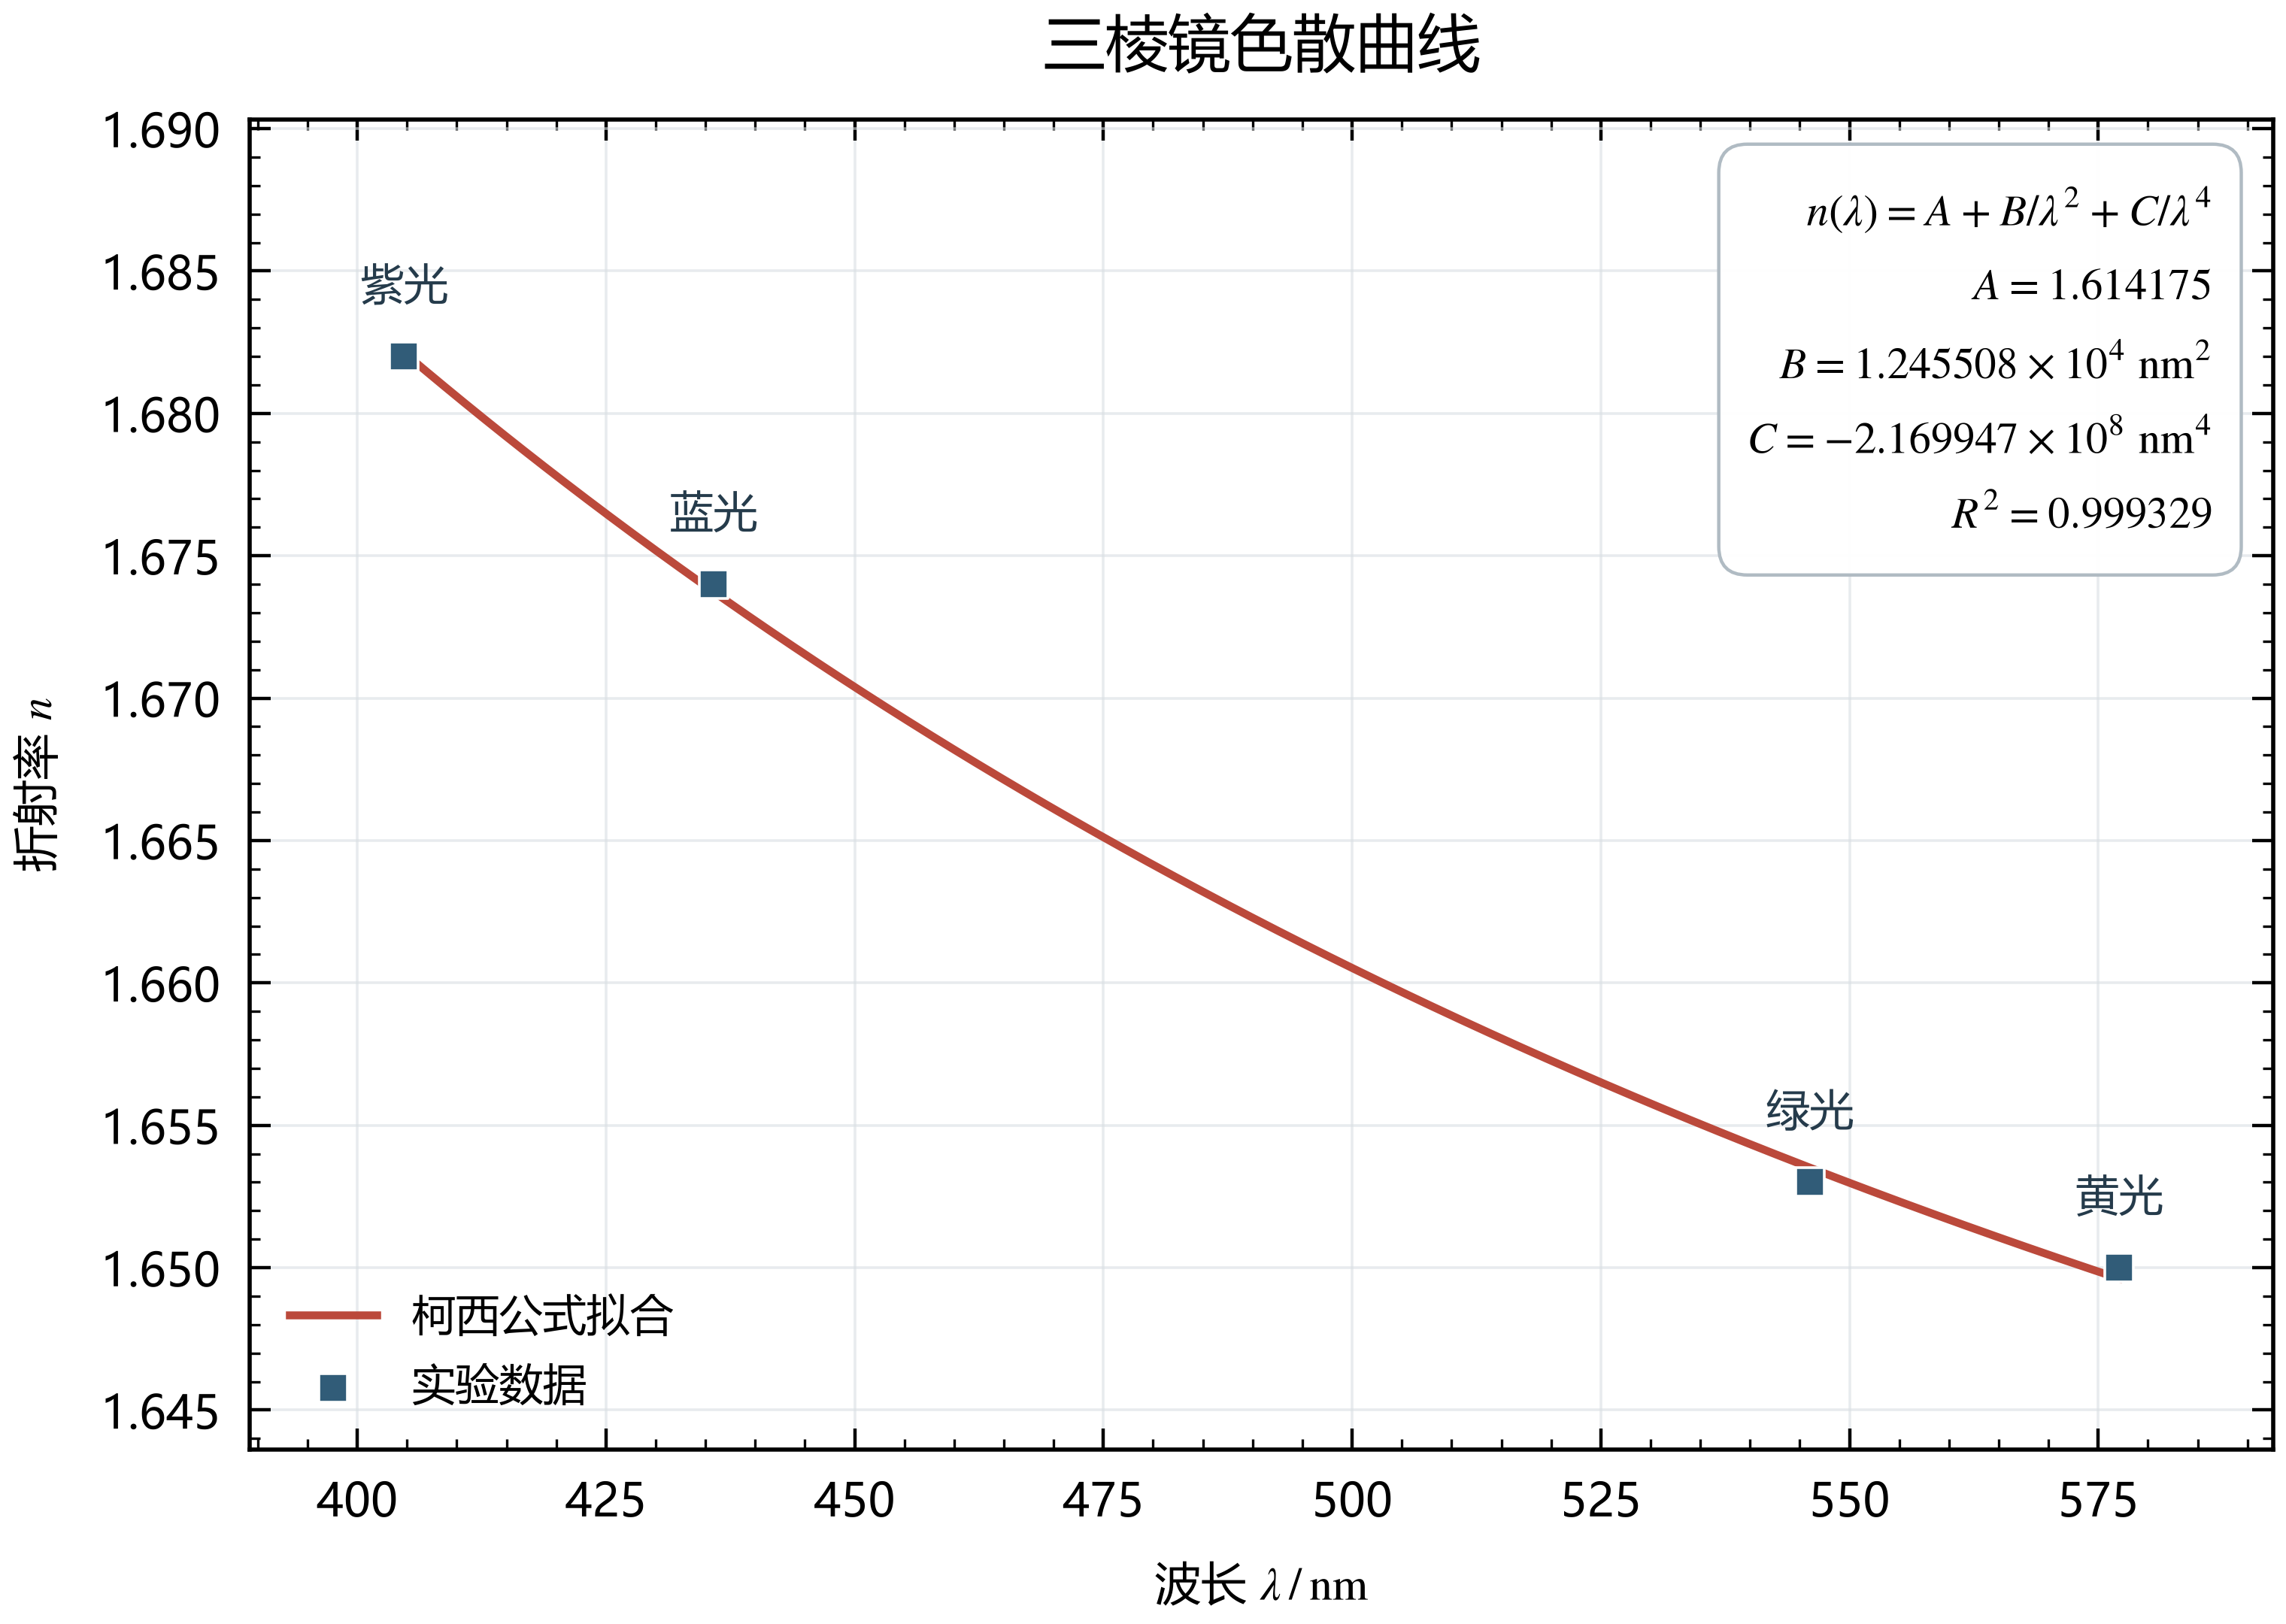
\includegraphics[width=0.6\textwidth]{figures/图5.png}
      \caption{三棱镜色散曲线}
    \end{figure}

  \subsection{误差分析（10分）}
  
    \subsubsection{分光计的调整与使用}
    三棱镜顶角测量的误差主要来源于以下几个方面：
    \begin{enumerate}
      \item 刻度盘中心与转轴中心不重合会产生偏心误差。双游标读数取平均可减小其影响，但仍存在刻度及仪器装配误差。
      \item 瞄准、微调及读数差异会引入随机误差。本实验 $u_a\approx0.71'$、$u_b\approx0.58'$，二者处于同一量级，重复测量的离散性与仪器允差的影响均不可忽略。
      \item 主尺与游标刻线具有一定宽度，其重合位置的判断受照明和观察位置影响，可能产生读数偏差。
      \item 三棱镜反射面上的灰尘或指纹会使反射像变暗、模糊，增大反射像与分划板刻线重合时的瞄准误差。
      \item 望远镜、平行光管及载物台调节不充分会引入测角偏差，微调或锁紧时的位置变化也会影响测量结果。
    \end{enumerate}

    \subsubsection{棱镜偏向角特性}
    误差主要来源于以下几个方面：
    \begin{enumerate}
      \item 分光计调焦、消视差或调平不充分，会影响谱线清晰度和测角准确性。
      \item 谱线在最小偏向位置附近移动时，转折点的判断难度较大，转动过快或跟踪不及时均会使得误差偏大。
      \item 狭缝宽度、旋钮空程和锁紧时的位置变化均会影响瞄准；移去三棱镜时碰动仪器，还可能改变入射光方向的测量基准。
      \item 游标读数及刻度误差不能完全消除。此外，顶角和最小偏向角的测量偏差都会影响折射率结果。
    \end{enumerate}

\section{实验探讨与思考题（10分）}

  \subsection{实验探讨}

    本次实验使我体会到，分光计的调焦、消视差和调平都十分重要，前期调整是否充分会直接影响后续测量。
    操作时应分清粗调、微调与锁紧旋钮的作用，缓慢调节，耐心跟踪谱线并确认最小偏向位置。

    三棱镜的放置应符合折射光路，使光线从两个光学面入射和出射，避免从粗糙面出射。
    寻找谱线时，可结合光路和刻度判断大致方位；利用双游标读数约相差$180^\circ$的关系检查读数，也能提高效率，
    但仍须分别实读两个游标。

  \subsection{思考题}

    \subsubsection{测量时如何确定最小偏向角的位置？}

    首先调好分光计，放置三棱镜，用望远镜找到待测颜色的折射谱线，并使其保持在视野内。
    随后缓慢转动承载三棱镜的载物台，即缓慢改变光线的入射角，同时配合转动望远镜跟踪谱线，观察其移动方向。
    本次实验的摆放条件下，我缓慢逆时针转动载物台，当谱线移动到某一位置后开始反向，
    即向顺时针方向移动时，反向前的转折位置就是最小偏向角位置。

    接近转折点时应减小转动幅度，可在其两侧小幅往返确认，最后将望远镜的竖直叉丝对准转折位置处的谱线中心，
    待稳定后锁牢三棱镜的载物台，读取左右两个游标。
    

    \subsubsection{另外设计一种测量三棱镜折射率的方法。}

    可采用掠入射法。设三棱镜两光学面$AB$、$AC$之间的顶角为$A$，单色光在$AB$面的入射角为$i$，
    棱镜内两次折射对应的角度分别为$r$、$r'$，从$AC$面射出的光线与该面法线的夹角为$\psi$。
    近似取空气折射率为1，根据折射定律和几何关系，有
    \[
    \sin i=n\sin r,\qquad
    n\sin r'=\sin\psi,\qquad
    r+r'=A
    \]
    当光线沿$AB$面掠入射，即$i\to90^\circ$时，$n\sin r=1$，因此
    \[
    \sin\psi=n\sin(A-r)
    =\sin A\sqrt{n^2-1}-\cos A
    \]
    整理得
    \[
    \boxed{n=\sqrt{1+\left(\frac{\cos A+\sin\psi}{\sin A}\right)^2}}
    \]

    实验时先测得三棱镜顶角$A$，将单色光源放在$AB$面的延长线方向，并在光源前放置毛玻璃形成扩展光源，
    使到达棱镜的光线包含接近掠入射的光线。用望远镜从$AC$面观察出射光，可看到由出射极限方向形成的明暗分界线，
    将竖直叉丝对准该分界线，记录双游标读数。保持载物台及三棱镜不动，再利用自准直法确定$AC$面的法线方向并记录双游标读数，
    两方向的夹角即为出射极限角$\psi$。将$A$和$\psi$代入上式，即可求得该单色光对应的折射率。

    该方法以掠入射所对应的出射极限角为测量依据，无需寻找最小偏向位置；
    实际测量时应保证明暗分界线清晰，并准确确定出射面的法线方向。

\vspace*{\fill} % 使下面内容在页面底部显示
\noindent
\begin{minipage}{\textwidth}
  注意事项：

  \begingroup
    \setlength{\leftskip}{2em} % 1--4整体向右缩进两个汉字宽度
    1. 用PDF格式上传“实验报告”，文件名：学生姓名+学号+实验名称+周次。

    2. “实验报告”必须递交在“学在浙大”本课程内对应实验项目的“作业”模块内。

    3. “实验报告”成绩必须在“浙江大学物理实验教学中心网站”-“选课系统”内查询。

    4. 教学评价必须在“浙江大学物理实验教学中心网站”-“选课系统”内进行，学生必须进行教学评价，才能看到实验报告成绩，教学评价须在本次实验结束之后3天内进行。\par
  \endgroup

  \begin{center}
    {\CJKfontspec[AutoFakeBold=2.5]{SimSun}\bfseries 浙江大学物理实验教学中心制}
  \end{center}
\end{minipage}

\end{document}
